\documentclass[11pt]{article}
\title{Symmetry 9}
\author{https://github.com/heptagons/lenses}
\date{2024/1/13}

\usepackage{graphicx}

\usepackage[margin=0.75in]{geometry}
\usepackage{float} % {figure}{H}
\usepackage{amsmath} % \dfrac

\def\mathbi#1{\textbf{\em #1}}

\begin{document}

\maketitle
\begin{abstract}
Symmetry 9
\end{abstract}

\section{Rhombi}

\begin{table}[H]
\begin{center}
\begin{tabular}{|c|c c| c | l | c |}
\hline
Rhombus & $\theta_1$ & $\theta_2$ & Area & Symmetry \\ \hline\
$\mathbi{a}$ & $\alpha/2$ & $2\alpha/2$  & $\sin(\alpha)$  & $R_3(\frac{1}2,1)$ \\[0.5ex]
\hline
$\mathbi{b}$ & $\beta/2$ & $4\beta/2$    & $\sin(2\beta)$  & $R_5(\frac{1}2,2)$ \\[0.5ex]
$\mathbi{c}$ & $2\beta/2$ & $3\beta/2$   & $\sin(\beta)$   & $R_5(1,\frac{3}2)$ \\[0.5ex]
\hline
$\mathbi{d}$ & $\gamma/2$ & $6\gamma/2$  & $\sin(3\gamma)$ & $R_7(\frac{1}2,3)$ \\[0.5ex]
$\mathbi{e}$ & $2\gamma/2$ & $5\gamma/2$ & $\sin(\gamma)$  & $R_7(1,\frac{5}2)$ \\[0.5ex]
$\mathbi{f}$ & $3\gamma/2$ & $4\gamma/2$ & $\sin(2\gamma)$ & $R_7(\frac{3}2,2)$ \\[0.5ex]
\hline
$\mathbi{g}$ & $\delta/2$ & $8\delta/2$  & $\sin(4\delta)$ & $R_9(\frac{1}2,4)$ \\[0.5ex]
$\mathbi{h}$ & $2\delta/2$ & $7\delta/2$ & $\sin(\delta)$  & $R_9(1,\frac{7}2)$ \\[0.5ex]
$\mathbi{a}$ & $3\delta/2$ & $6\delta/2$ & $\sin(3\delta)=\sin(\alpha)$ & $R_9(\frac{3}2,3)$ \\[0.5ex]
$\mathbi{i}$ & $4\delta/2$ & $5\delta/2$ & $\sin(2\delta)$ & $R_9(2,\frac{5}2)$ \\[0.5ex]
\hline
\end{tabular}
\caption{Rhombi for symmetries $\{3,5,7,9\}$ internal angles $\theta_1 < \theta_2$ ($\theta_1 + \theta_2 = \pi$) and areas. $\alpha = 2\pi/3$, $\beta = 2\pi/5$, $\gamma = 2\pi/7$ and $\delta = 2\pi/9$ $(3\delta = \alpha)$.} 
\label{tbl:bc-angles}
\end{center}
\end{table}

\subsection{Stars from rhombi}

\begin{figure}[H]
\centering
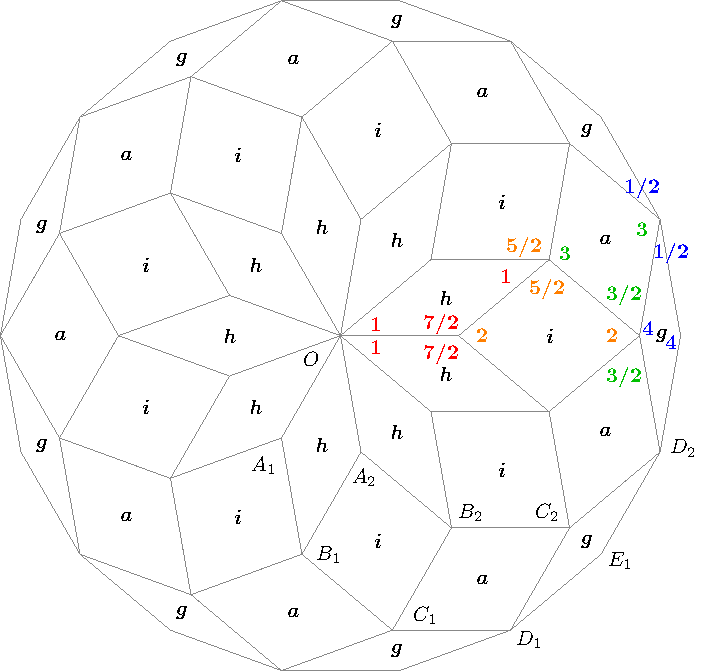
\includegraphics[scale=1]{rhombi-9}
\caption{The symmetry $9$ four rhombi $\{h,i,a,g\}$ produce the four stars $\{S_G,S_H,S_I,S_J\}$ respectivelly with areas $\{9(h+i+a+g),9(h+i+a),9(h+i),9h)\}$ .}
\label{fig:rhombi-9}
\end{figure}

\section{Hexagons}

\subsection{Hexagons from stars}

\begin{figure}[h]
\centering
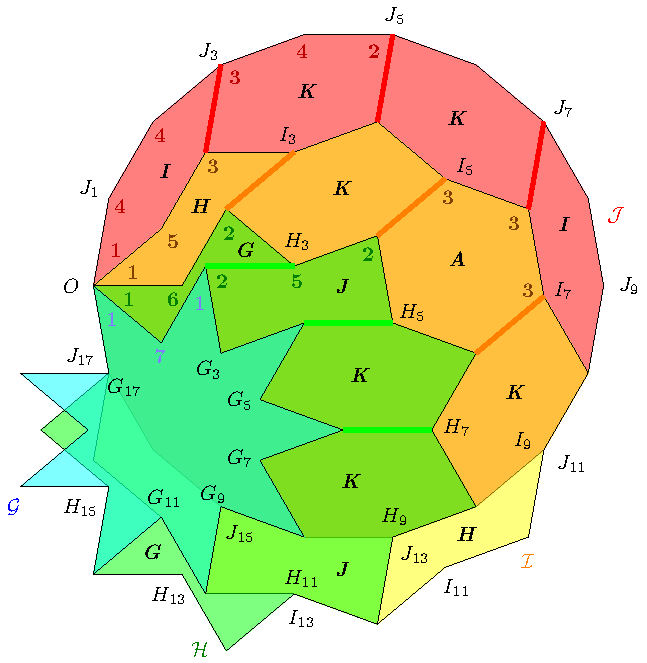
\includegraphics[scale=1]{hexagons-9}
\caption{Symmetry $9$ stars $\{S_G,S_H,S_I,S_J\}$ dissected with vectors to get symmetry-9 hexagonal hexagons.}
\label{fig:hexagons-9}
\end{figure}

Figure \ref{fig:hexagons-9} show the disposition of the symmetry $9$ four stars $\{S_G,S_H,S_I,S_J\}$. We denote the $18$ vertices of every star as $\{X_0,X_1,...,X_{17}\}$ where $X = \{G,H,I,J\}$. Only some vertices are labeled in the figure. First we make coincident at vertice $O$ all the vertices $G_0,H_0,I_0,J_0$. With the center at $O$ we rotate star $S_H$ to make coincident vertices $G_{17}$ and $H_{17}$. Similarly we rotate stars $S_I$ and $S_J$ to make coincident vertices $G_{17}$ and $I_{17}$ and vertices $G_{17}$ and $J_{17}$. The rotations also joined another different vertices.

First we add three new edges (in red) joining the stars $S_G$ and $S_H$ vertices: $\overline{G_3H_2}$, $\overline{G_5H_4}$ and $\overline{G_7H_6}$ dissecting the red region into four hexagons, two of them essentially different. The three consective angles of the two hexagons are shown: $(\textbf{1,4,4})$ and $(\textbf{3,4,2})$.

Then we add three new edges (in orange) joining the stars $S_H$ and $S_I$ vertices: $\overline{H_3I_2}$, $\overline{H_5I_4}$ and $\overline{H_7I_6}$ dissecting the orange region into four hexagons, two of them new. The three consective angles of the the two hexagons are show: $(\textbf{1,5,3})$ and $(\textbf{3,3,3})$.

Finally we add three more edges (in green) joining the stars $S_I$ and $S_J$ vertices:
$\overline{I_3J_2}$, $\overline{I_5J_4}$ and $\overline{I_7J_6}$ dissecting the green region into four hexagons, two of them new. The three consective angles of the the two hexagons are show: $(\textbf{1,6,2})$ and $(\textbf{2,5,2})$.

The three consecutive angles of the hexagons are of the form $(a,b,c)$ where $a+b+c = 9$. Table \ref{tbl:hexagons-angles}

\begin{table}[H]
\begin{center}
\begin{tabular}{| c | c c c | l | }
\hline
Hexagon & $\textbf{a}$ & $\textbf{b}$ & $\textbf{c}$ & Details \\ \hline\
$H_9(1,1)$ & 1 & 1 & 7 & self-intersecting \\[1.1ex] \hline
$H_9(1,2)$ & 1 & 2 & 6 & Lense \textbf{\em H$^+$}\\[1.1ex] \hline
$H_9(1,3)$ & 1 & 3 & 5 & Lense \textbf{\em H} \\[1.1ex] \hline
$H_9(1,4)$ & 1 & 4 & 4 & Lense \textbf{\em G} \\[1.1ex] \hline
$H_9(2,2)$ & 2 & 2 & 5 & Lense \textbf{\em J} \\[1.1ex] \hline
$H_9(2,3)$ & 2 & 3 & 4 & Lense \textbf{\em I} \\[1.1ex] \hline
$H_9(3,3)$ & 3 & 3 & 3 & Lense \textbf{\em A} equal to $H_3(1,1)$ \\[1.1ex] \hline
\end{tabular}
\caption{Symmetry $9$ hexagons with angles factors $a \leq b \leq c$.} 
\label{tbl:hexagons-angles}
\end{center}
\end{table}




\end{document}

